\documentclass{ctexart}
\usepackage{EC}
\begin{document}
\section{铝及其化合物}
\subsection{单质铝}
\subsubsection{单质铝的制备}
丹麦科学家H. C. Oersted的利用稀的钾汞齐与\ce{AlCl3}反应第一次分离出不纯的金属铝.1854年,H. St. C. Deville和R. W. Bunsen各自通过熔融\ce{NaAlCl4}的电解得到了金属铝:
\begin{center}
    \ce{2NaAlCl4 ->T[电解] 2NaCl + 2Al + 3Cl2}
\end{center}

\indent 当时,这种金属极其珍贵,以至于在1855年的巴黎博览会上它与王冠上的宝石在一起展出.Louis Napoleon III在国宴上还使用铝制刀叉餐具.\\
\indent 在19世纪末,由于发电机的改进,人们拥有了更廉价的电力;此外,P. L. T. Héroult和C. M. Hall于1886年分别发明了将\ce{Al2O3}溶解在\ce{Na3AlF6}(即冰晶石)中电解的方法:
\begin{center}
    \ce{2Al2O3 ->T[\ce{Na3AlF6}][电解] 2Al + 3O2}
\end{center}
然而,冰晶石的产量是远不足以供应此法所需的.因此可以采取以下方法合成人工冰晶石:
\begin{center}
    \ce{6HF + Al(OH)3 + 3NaOH -> Na3AlF6 + 6H2O}
\end{center}
电解生产铝的耗电量是巨大的.因此,最近几年以来,中国是世界上生产铝单质最多的国家,占全球总产量的一半以上.
\subsubsection{单质铝的性质与用途}
纯铝是一种银白色金属,具有许多优秀的性质.它轻而无毒,有着好看的外观,并能做出光泽度高的表面.它具有高的热导率和电导率,极好的抗腐蚀性\footnote{铝的抗腐蚀性来源于其表面形成的\ce{Al2O3}氧化膜,这与铝在电化学序列中排在较活泼的位置并不矛盾.},无磁性.铝的延性仅次于金,展性也是所有金属中的前列.它的许多合金具有高机械强度和高抗张强度.\\
\indent 正因如此,铝合金被用于各种小型的高强度结构,例如门窗,车辆,易拉罐等等各种设备中.飞机的主要材料也是铝合金,因为它轻且强度高.此外,铝的高导电性也使其成为架空电线的主材(埋入地面的线材则以铜线为主).
\subsubsection{单质铝的化学性质}
尽管铝的化学性质是活泼的,但由于表面\ce{Al2O3}氧化膜的阻挡使其对\ce{H2O}和稀酸比较稳定.\\
\indent 我们在高中化学中就已经学过铝是两性的.这意味着它既可以与酸反应也可以与碱反应:
\begin{center}
    \ce{2Al + 6HCl -> 2AlCl3 + 3H2}\\
    \ce{2Al + 2NaOH + 6H2O -> 2Na[Al(OH)4] + 3H2}
\end{center}
关于这些产物的性质,我们到对应的部分再详细描述.
\subsection{铝的氢化物和相关的配合物}
\paragraph{\ce{AlH3}}
与\ce{B}不同的是,\ce{Al}(包括所有IIIA族更重的金属元素)几乎只能形成简单的氢化物.
\begin{substance}[\ce{AlH3}]
    氢化铝,化学式为\ce{AlH3},是易挥发的无色至白色针状晶体,熔点为$150\tc$.
\end{substance}
\ce{AlH3}最好在控制条件下将\ce{LiAlH4}与\ce{AlCl3}反应得到:
\begin{center}
    \ce{3LiAlH4 + AlCl3 ->T[\ce{Et2O}] 4AlH3 + 3LiCl}
\end{center}
为了避免\ce{AlH3(Et2O)_n}的出现,需要使\ce{LiAlH4}过量并加入一些\ce{LiBH4}.\\
\indent \ce{AlH3}最常见的晶型$\alpha$-\ce{AlH3}与\ce{B2H6}有明显的区别.其中\ce{Al}处于六个\ce{H}原子构成的八面体中心,八面体之间共顶点连接.然而,\ce{AlH3}和\ce{BH3}一样容易接受Lewis碱的配位,并且还可以形成\ce{B}所不能形成的五配位结构:
\begin{center}
    \ce{LiAlH4 + Me3NHCl ->T[Et2O] Me3NAlH3 + LiCl + H2}\\
    \ce{Me3NAlH3 + Me3N -> (Me3N)2AlH3}
\end{center}
上述两种配合物的结构如下:
\bichemfig{AlH3(NMe3)}{1}{\ce{AlH3(NMe3)}的结构}{AlH3(NMe3)2}{1}{\ce{AlH3(NMe3)2}的结构}{\ce{AlH3}与\ce{NMe3}的配合物的结构}
\paragraph{\ce{LiAlH4}}
\ce{AlH3}最重要的衍生物就是\ce{LiAlH4}.这种白色的晶状固体在干燥的空气中是稳定的,但遇到潮湿的质子溶剂或有机官能团就体现出强还原性.\ce{LiAlH4}易溶于醚中,因此一般在各种醚中使用.\\
\indent \ce{LiAlH4}主要通过下面的方法制备:
\begin{center}
    \ce{4LiH + AlCl3 ->T[\ce{Et2O}] LiAlH4 + 3LiCl}
\end{center}
也可以通过在高压下用单质直接化合得到钠盐后交换得到:
\begin{center}
    \ce{Na + Al + 2H2 ->T[\ce{THF}][$140\tc$,350\ atm] NaAlH4}\\
    \ce{NaAlH4 + LiCl ->T[\ce{Et2O}] NaCl + LiAlH4}
\end{center}
尽管看上去\ce{LiAlH4}是离子化合物\ce{[Li]+[AlH4]-},但在晶体中\ce{Li}与周围的四个\ce{H}之间的距离小于$200\text{ pm}$,即小于\ce{LiH}中相应的距离,因此认为\ce{LiAlH4}是共价晶体似乎更加合适.
\paragraph{其它氢配合物}
已经发现的其它氢配合物包括\ce{Li3AlH6}等等.这些物质都具有强还原性,在有机化学中常用它们作为还原剂,例如\ce{DIBAL}等等试剂.\\
\indent 一种重要的氢化物配合物是\ce{Al(BH4)3},这种无色液体可以用于火箭燃料,航空油添加剂等.它最好通过无溶剂的置换反应来制备:
\begin{center}
    \ce{AlCl3 + 3NaBH4 -> 3NaCl + Al(BH4)3}
\end{center}
\ce{Al(BH4)3}不稳定,容易受热分解生成双核配合物\ce{Al2B4H18}(也许写成\ce{Al2H2(BH4)4}更好):
\begin{center}
    \ce{2Al(BH4)3 ->T[$70\tc$] Al2B4H18 + B2H6}
\end{center}
两者中的\ce{BH4-}都是双齿配体,并且是流变的,因而无法分辨参与配位的\ce{H}和端基\ce{H}.在室温下,\ce{Al(BH4)3}定量地与\ce{Al2Me6}反应生成\ce{MeAl(BH4)2}:
\begin{center}
    \ce{4Al(BH4)3 + Al2Me6 ->T[回流] 6MeAl(BH4)2}
\end{center}

\indent 下面给出了上述三者的结构示意图.
\begin{figure}[H]
    \centering
    \subfigure[\ce{Al(BH4)3}的结构]{
        \begin{minipage}[b]{.31\linewidth}
            \centering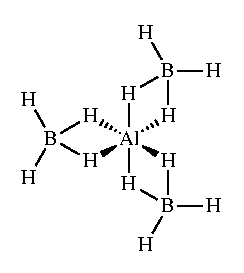
\includegraphics{picture/Al(BH4)3.eps}
        \end{minipage}
    }
    \subfigure[\ce{Al2B4H18}的结构]{
        \begin{minipage}[b]{.31\linewidth}
            \centering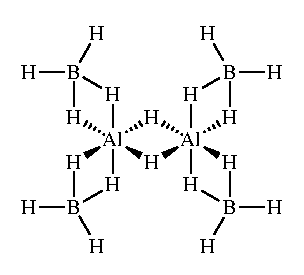
\includegraphics{picture/Al2B4H18.eps}
        \end{minipage}
    }
    \subfigure[\ce{MeAl(BH4)2}的结构]{
        \begin{minipage}[b]{.31\linewidth}
            \centering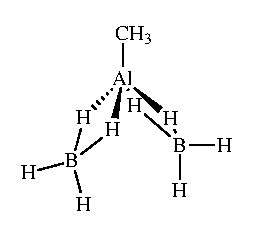
\includegraphics{picture/MeAl(BH4)2.eps}
        \end{minipage}
    }\caption{\ce{Al}的\ce{BH4-}配合物的结构}
\end{figure}
\subsection{铝的卤化物和相关的配合物}
\paragraph{一卤化物\ce{AlX}}
\ce{Al}的一卤化物仅在气相中以分子的形式短暂存在.这是因为\ce{AlX3}的强大的稳定性使得它们在凝聚相中容易发生歧化:
\begin{center}
    \ce{3AlX -> 2Al + AlX3}
\end{center}
这与之后的\ce{Ga,In}和\ce{Tl}是不同的.\\
\indent 将\ce{AlCl}通入\ce{CH3OH}中即可结晶得到\ce{AlCl4.4CH3OH}.
\paragraph{\ce{AlF3}及其衍生物}
与其它\ce{AlX3}不同,\ce{AlF3}最好由\ce{HF}对\ce{Al2O3}的氟化而制备(其它则由单质直接化合得到):
\begin{center}
    \ce{Al2O3 + 6HF -> 2AlF3 + 3H2O}
\end{center}
\ce{AlF3}与其它的\ce{AlX3}的物理性质有着显著的差异.
\begin{table}[H]
    \centering
    \begin{tabular}{ccccc}
        \hline
        性质    &\ce{AlF3}  &\ce{AlCl3} &\ce{AlBr3} &\ce{AlI3}\\\hline
        熔点/$\tc$  &$1290$ &$192.4$    &$97.8$     &$189.4$\\
        $\Delta H_\text{f}^\ominus/\kJm$    &$-1498$    &$-707$ &$-527$ &$-310$\\\hline        
    \end{tabular}
\end{table}
熔点或升华点的差异主要来源于结构上的不同.因此,我们先来研究\ce{AlF3}的晶体结构.
\bichemfig{AlF3-1}{0.1}{\ce{AlF3}的晶胞示意图}{AlF3-2}{0.1}{\ce{AlF3}沿$\dfrac23\mbf{a}+\dfrac13\mbf{b}-\dfrac16\mbf{c}$方向的投影}{\ce{AlF3}的晶体结构}
其中每个\ce{Al}被\ce{F}八面体配位,每个\ce{F}由两个八面体共顶点而共用,形成$1:3$的比例.若非畸变,这一结构事实上描述的就是\ce{ReO3},而轻微的畸变使得\ce{AlF3}退化为了三方晶系.事实上,$\alpha$-\ce{AlH3}也具有与\ce{AlF3}相同的结构.\\
\indent 相应的,\ce{Al}的\ce{F}配合物中广泛存在由\ce{F}桥连的\ce{\{AlF6\}}八面体.\\
\indent 我们先来看冰晶石\ce{Na3AlF6}.看起来这其中有分立的\ce{[AlF6]^3-}离子,\ce{\{AlF6\}}单元也确实是独立的,但\ce{Al-F}键与其它\ce{M-F}键并无不同.这使得我们\tbf{也许}\footnote{Greenwood提出的此观点未免有些离奇.}可以从另一种角度考虑它的结构,即\ce{Na+}和\ce{Al^3+}共同填入\ce{F-}形成的空隙中.事实上,这一结构与\ce{CaTiO3}有着密切关系,\ce{Al}和$\dfrac13$的\ce{Na}填入八面体空隙,$\dfrac23$的\ce{Na}填入12配位的位置.只不过这畸变实在是太过严重,以至\ce{Na3AlF6}事实上是单斜晶系的.
\bichemfig{Na3AlF6-1}{0.1}{\ce{Na3AlF6}的晶胞示意图}{Na3AlF6-2}{0.1}{\ce{Na3AlF6}沿$\mbf{a}+\mbf{b}$方向的投影}{\ce{Na3AlF6}的晶体结构}
八面体顶点间的共用将导致\ce{Al}与\ce{F}的比例偏离$1:6$,而向$1:3$靠近.例如\ce{K2AlF5}中的\ce{\{AlF6\}}八面体共用顶点形成长链,使得$\ce{Al}:\ce{F}=1:5$;\ce{KAlF4}中的\ce{\{AlF6\}}八面体共用顶点形成二维层状结构,使得$\ce{Al}:\ce{F}=1:4$.需要注意的是,后者中不存在\ce{\{AlF4\}}四面体,不要被化学式所蒙骗.
\bichemfig{K2AlF5}{0.1}{\ce{K2AlF5}的晶胞示意图}{KAlF4}{0.1}{\ce{KAlF4}的晶胞示意图}{\ce{Al}的其它氟配合物的晶体结构}
更复杂的计量比对应着更复杂的共用方式.在\ce{Na5Al3F14}中,$\dfrac13$的\ce{\{AlF6\}}共用赤道\ce{F},而$\dfrac23$的\ce{\{AlF6\}}共用顶点\ce{F}.
\bichemfig{Na5Al3F14-1}{0.1}{\ce{Na5Al3F14}的晶胞示意图}{Na5Al3F14-2}{0.1}{\ce{Na5Al3F14}沿$c$轴的投影图}{\ce{Na5Al3F14}的晶体结构}
\paragraph{\ce{AlCl3}及其衍生物}
制备无水\ce{AlCl3}可以通过单质的直接化合,亦可以通过还原氯化\ce{Al2O3}的方法:
\begin{center}
    \ce{2Al + 3Cl2 -> 2AlCl3}\\
    \ce{Al2O3 + 3C + 3Cl2 -> 2AlCl3 + 3CO}
\end{center}

\indent \ce{AlCl3}晶体的结构与\ce{AlF3}并无明显区别.然而,熔化成液体后它将变为\ce{Al2Cl6}分子,并且在温度不高时的气相也以此形式存在,而在高温下离解为\ce{AlCl3}分子.
\bichemfig{Al2Cl6}{1}{\ce{Al2Cl6}的结构}{AlCl3}{1}{\ce{AlCl3}的结构}{\ce{AlCl3}及其二聚体的结构}
$\ce{NaCl}-\ce{AlCl3}$熔体中存在\ce{[AlCl4]-},\ce{[Al2Cl7]-}等离子.电解这一熔体制备\ce{Al}单质的能耗相比冰晶石-氧化铝法更小,然而由于制备无水\ce{AlCl3}花费高昂,因此并不采取此法.
\bichemfig{AlCl4-}{1}{\ce{[AlCl4]-}的结构}{Al2Cl7-}{1}{\ce{[Al2Cl7]-}的结构}{\ce{AlCl3}与\ce{Cl-}形成的配离子的结构}
\ce{AlCl3}是常用的Lewis酸.它能夺取某些烷基氯化物中的\ce{Cl}形成碳正离子:
\begin{center}
    \ce{Ph3CCl + AlCl3 -> [Ph3C]+[AlCl4]-}
\end{center}
它也可以与酰基氯化物\ce{RCOCl}反应形成\ce{O}-配合物或酰基正离子\ce{[RCO]+[AlCl4]-}.\\
\indent 另一个复杂一些的例子是\ce{AlCl3}在\ce{POCl3}溶剂中的反应.我们在介绍\ce{POCl3}时已经提到过发生的反应:
\begin{center}
    \ce{4AlCl3 + 6POCl3 -> [Al(OPCl3)6]^3+ + 3[AlCl4]-}
\end{center}

\indent \ce{AlCl3}也可以将非金属氟化物转变为氯化物,例如:
\begin{center}
    \ce{BF3 + AlCl3 -> AlF3 + BCl3}
\end{center}
一般而言,这样的复分解反应最终总是使电负性最大的元素和电正性最大的元素结合在一起.\\
\indent 在工业上,\ce{AlCl3}主要作为Lewis酸催化各种烷基化/酰基化反应.一个典型的例子是染料工业上合成蒽醌:
\begin{center}
    \ce{2C6H6 + 2COCl2 ->T[\ce{AlCl3}] C14H8O2 + 2HCl}
\end{center}
\paragraph{\ce{AlBr3}与\ce{AlI3}}
在固相和液相中,这两种物质都以二聚体\ce{Al2X6}的形式存在.除此之外,它们的性质事实上和\ce{AlCl3}有诸多类似之处,这里就不再介绍了.
\subsection{铝的氧化物和氢氧化物}
\subsubsection{\ce{Al2O3}}
\paragraph{刚玉$\alpha$-\ce{Al2O3}}
\ce{Al2O3}最稳定的形式为$\alpha$-\ce{Al2O3},即我们熟知的刚玉.刚玉具有极高的硬度,熔点,化学惰性和绝缘性,因此被作为磨料,耐火材料和陶瓷制品等而具有广泛的应用.\\
\indent 刚玉晶体中掺杂金属离子会使得其具有鲜明的颜色,因此可以作为宝石.
\begin{table}[H]
    \centering\begin{tabular}{ccccc}
        \hline
        掺杂    &\ce{Cr^{III}}  &\ce{Fe^{III}/Ti^{IV}}  &\ce{Cr^{III}/V^{III}}  &\ce{Cr^{III}/Ti^{IV}}\\\hline
        颜色    &红色   &蓝色   &绿色   &紫色\\\hline
        名称    &红宝石 &蓝宝石 &绿宝石 &紫水晶\\\hline
    \end{tabular}
\end{table}
高温煅烧\ce{Al(OH)3}即可制得刚玉.\\
\indent 刚玉中\ce{O}近似地做立方最密堆积,\ce{Al}有序地占据$\dfrac23$的八面体空隙.空隙与\ce{O}原子可以用如下记号关系表示:
\[\cdots AcBaCb\overline{AcBaCb}AcBaCb\cdots\]
因此也容易看出刚玉属于三方晶系,点阵形式为$R$心六方点阵.下面是刚玉的晶体结构示意图.
\bichemfig{alpha-Al2O3-1}{0.1}{$\alpha$-\ce{Al2O3}的晶胞沿$a$轴的投影图}{alpha-Al2O3-2}{0.1}{$\alpha$-\ce{Al2O3}的晶胞沿$c$轴的投影图}{$\alpha$-\ce{Al2O3}的晶体结构}
\paragraph{$\gamma$-\ce{Al2O3}}
\ce{Al2O3}的第二种晶型是密度较小的$\gamma$-\ce{Al2O3},由\ce{Al(OH)3}低温脱水得到.它是由缺陷的尖晶石结构,$24$个可用的阳离子位置中\ce{Al^3+}无序地占据$\dfrac{64}{3}$个.\\
\indent 由于其中存在数量相当的空隙,因此$\gamma$-\ce{Al2O3}可以作为催化剂或催化剂载体.
\paragraph{\ce{Al}表面的\ce{Al2O3}保护层}
我们前面提到\ce{Al}的相对惰性来源于其表面的\ce{Al2O3}保护层.这一保护层的\ce{Al2O3}为有缺陷的\ce{NaCl}型结构,\ce{Al}占据$\dfrac23$的八面体空隙.
\subsubsection{\ce{AlO(OH)}}
\paragraph{勃姆石$\gamma$-\ce{AlO(OH)}}
将\ce{NH3}水溶液加入冷的\ce{Al^3+}水溶液中,并将得到的白色胶状沉淀加热即可得$\gamma$-\ce{AlO(OH)}.
\paragraph{硬水铝石$\alpha$-\ce{AlO(OH)}}
这一晶型的\ce{AlO(OH)}存在于某些类型的粘土矿中,可以在高压下的稀\ce{NaOH}溶液中处理勃姆石得到.
\subsubsection{\ce{Al(OH)3}}
\paragraph{三羟铝石$\alpha$-\ce{Al(OH)3}}
三羟铝石在自然界中并不存在,但可以从冷的碱溶液中迅速沉淀得到:
\begin{center}
    \ce{2[Al(OH)4]- + CO2 -> 2Al(OH)3 + CO3^2- + H2O}
\end{center}
\paragraph{水铝石$\gamma$-\ce{Al(OH)3}}
水铝石则是常见得多的晶型,可以由热碱溶液中\ce{Al^3+}的沉淀或煮沸水解\ce{Al^3+}的盐得到.
\subsection{铝的复杂氧化物}
\subsubsection{尖晶石及其衍生物}
尖晶石是一大类化合物,其晶体结构以尖晶石矿\ce{MgAl2O4}为基准对阴阳离子进行更换得到.这种重要的晶体的结构如下:
\bichemfig{MgAl2O4-1}{0.1}{\ce{MgAl2O4}的晶胞示意图}{MgAl2O4-2}{0.1}{\ce{MgAl2O4}沿$a$轴的投影图}{\ce{MgAl2O4}的晶体结构}
尖晶石的结构可以看作\ce{O^2-}做立方最密堆积,\ce{Mg^2+}有序地占据$\dfrac18$的四面体空隙,\ce{Al^3+}有序地占据$\dfrac12$的八面体空隙.\\
\indent 尖晶石的晶胞可以划分为八个小立方体,分为两种.除去占据一半顶点的\ce{Mg^2+}之外,一种的内部为\ce{\{Al4O4\}}立方体,另一种的内部为\ce{\{MgO4\}}四面体.这两种小立方体交替排列形成了尖晶石.
\bichemfig{MgAl2O4-3}{1}{立方体I}{MgAl2O4-4}{1}{立方体II}{\ce{MgAl2O4}的晶体结构}
尖晶石型化合物都具有\ce{AB2O4}的化学式,并且大多数尖晶石的价态事实上为\ce{A^{II}B^{III}_2O4}.根据正离子占据空隙的不同,可以将尖晶石类化合物分为常式尖晶石和反式尖晶石两种.
\begin{enumerate}[label=\tbf{\arabic*.},topsep=0pt,parsep=0pt,itemsep=0pt,partopsep=0pt]
    \item \tbf{常式尖晶石}\\
        八面体空隙由三价正离子占据,四面体空隙由二价正离子占据,可以写作\ce{[A^{II}]_{$t$}[B^{III}_2]_{$o$}O4}.\\
        典型的具有常式尖晶石结构的晶体有\ce{MgAl2O4},\ce{Co3O4},\ce{CuCr2Te4}等等.
    \item \tbf{反式尖晶石}\\
        八面体空隙由二价正离子占据,四面体空隙由二价正离子和三价正离子共同占据,可以写作\ce{[B^{III}]_{$t$}[A^{II}B^{III}]_{$o$}O4}.\\
        典型的具有反式尖晶石结构的晶体有\ce{MgFe2O4},\ce{Fe3O4},\ce{TiMg2O4}等等.
\end{enumerate}
\indent 影响晶体采取常式尖晶石还是反式尖晶石的因素主要包括离子的半径与电荷,以及在八面体场和四面体场的稳定化能等.
\subsubsection{钠-$\beta$-氧化铝\ce{NaAl11O17}}
X-射线分析表明此晶体的结构与尖晶石结构接近,晶胞内的大部分原子精确地按尖晶石的结构排列.大的Na原子只是松散地与相等数目的氧原子一起堆积成平面,将尖晶石层隔开.
\bichemfig{NaAl11O17-1}{0.1}{\ce{NaAl11O17}的晶胞示意图}{NaAl11O17-2}{0.1}{\ce{NaAl11O17}沿$\mbf a+\mbf b$方向的投影图}{\ce{NaAl11O17}的晶体结构}
作为对比,以下是\ce{MgAl2O4}沿$\mbf a+\mbf b$方向的投影图.
\chemfig{MgAl2O4-5}{0.125}{\ce{MgAl2O4}沿$\mbf a+\mbf b$方向的投影图}
\subsection{铝的金属有机化合物}
铝的三烷基化合物和三芳基化合物是高度活性的,无色的易挥发液体或是能在空气中自燃的低熔点固体,若遇水则激烈反应,所以应谨慎使用并作好适当的预防措施.这些化合物与\ce{BR3}和\ce{BAr3}不同,它们常常以二聚体的形式存在.
\chemfig{Al2Me6}{1}{\ce{AlMe3}的二聚体结构}

\end{document}